\section{Study 2: Coordinate Banks and Original Characterization}
\label{app:characterization}
The original coordinate characterization was specified after excluded development comparisons. It completed 72 model/readout/domain cells, 120 structural split records and 48 $C_7/D_4$ field-comparison cells. The results below are reviewed descriptive aggregates. Original source flags and failed decisions remain unchanged in the release archive. Because these evaluation outputs have been inspected, they cannot serve as untouched data for later method selection.

\paragraph{Data and information conditions.}
The same six pinned base models and four readouts use training-only $q=16$ coordinates, with BF16 model extraction and F64 coordinate analysis. New extraction comprises 41,728 rows per model: 896 $C_7$, 512 $D_4$ and 40,320 $S_3$ rows, including separately charged support. The C7/D4 state vocabularies are seen in construction. S3 also retains its six abstract assignment states, but its new-entity and joint strata hold out entity names/triples. Unseen-composite supervision concerns actions, not new C7/D4 states or independently authored grammar roots. Coordinate fields receive source coordinates and the requested action. The separate decoded-centroid benchmark has training state labels and the known action table, but decodes the source at evaluation. In contrast, the legacy prediction contrasts in \cref{tab:characterization-intervals} select oracle-source category/retention controls (and an input-metadata potential for S3) on validation; they are not the decoded-source benchmark.

\paragraph{Losses and aggregation.}
The characterization normalizes squared errors by common training-only energy scales; the historical $D$ in \cref{eq:D} averages per-row target-normalized errors. Values across the two studies are therefore not interchangeable. Writing $\bar z_{\rm tr}$ for the training mean, prediction uses $E_z=\mathbb{E}_{\rm tr}\norm{z-\bar z_{\rm tr}}_2^2$. For two paraphrases ordered by their registered identifiers, set $u=z_{p_0}-z_{p_1}$; transport uses $E_u=\mathbb{E}_{\rm tr}\norm{u}_2^2$, without recentering. The row losses are $\norm{\widehat z_g-z_{g(i)}}_2^2/E_z$ and $\norm{\widehat u_g-u_{g(i)}}_2^2/E_u$. Validation and evaluation retain only changed-state pairs $g(i)\ne i$. All-element fitting still uses all training pairs, including identity/fixed points; generator fitting and selection use only primitives. Historical nonidentity-action averages can include D4 fixed points. Prediction and transport thus differ in denominator as well as target. These original coordinate summaries pool changed-state pairs; the later equal-action aggregation is explicitly distinguished in \cref{app:aggregation-contract}. Models and readouts form a fixed panel, averaged within family/entity units. The resampling units are $64\times1$ for $C_7/D_4$, $64\times16$ for jointly new $S_3$ contexts/entities, $64\times24$ for new contexts, and $48\times16$ for new entities. Independently resampled family/entity indices give the crossed $S_3$ sensitivities. No new superiority, equivalence or multiplicity-controlled decision is made.
\begin{table}[htbp]\centering\small
\begin{tabular}{llrrr}\toprule
Domain / split & Endpoint & Baseline minus linear & Lower & Upper \\
\midrule
$C_7$, new context & prediction & -0.002887 & -0.003290 & -0.002495 \\
$C_7$, new context & context & 0.011485 & 0.009997 & 0.013087 \\
$D_4$, new context & prediction & 0.019612 & 0.014730 & 0.025945 \\
$D_4$, new context & context & 0.060918 & 0.049883 & 0.072920 \\
$S_3$, context & prediction & -0.000487 & -0.000791 & -0.000249 \\
$S_3$, context & context & 0.000177 & 0.000010 & 0.000348 \\
$S_3$, entity & prediction & 0.000673 & 0.000443 & 0.000927 \\
$S_3$, entity & context & 0.000739 & 0.000542 & 0.000978 \\
$S_3$, joint & prediction & 0.000460 & 0.000262 & 0.000673 \\
$S_3$, joint & context & 0.000154 & -0.000017 & 0.000338 \\
\bottomrule\end{tabular}
\caption{All ten original characterization contrasts with frozen 95\% percentile sensitivity intervals (10,000 draws, seed 314159). Positive favors linear. Prediction uses oracle-source category/retention controls, plus the $S_3$ input-metadata potential, selected on validation; context uses scalar retention. Prediction and context have different training-energy denominators. Fixed-panel sensitivities do not certify significance, equivalence, coverage or an old power gate.}
\label{tab:characterization-intervals}\end{table}


\paragraph{Prediction and compact category controls.}
All-element direct ridge versus full-kernel means are $0.014900/0.004626$ for $C_7$ and $0.041349/0.020916$ for $D_4$. A training-centroid displacement predictor uses
\[
 \widehat z_g=z+\mu_{g(\widehat i(z))}-\mu_{\widehat i(z)},
\]
where $\widehat i$ is the nearest training centroid. Source decoding is perfect in all $C_7/D_4$ field conditions. C7's error is $0.012013$, better than ridge on average but in only 9/24 individual conditions; D4's $0.062349$ is worse on average and improves only 2/24. Centroids occupy 112 and 64 floating-point coordinates, respectively, plus the exact integer action table and decoding logic. This is a strong cheap control under additional construction labels, not a strict match to label-free field information. Evaluating a known composite label after one source decode is also distinct from repeated primitive evaluation with re-decoding at each intermediate output; the former cannot certify the latter.

\begin{figure}[t]\centering
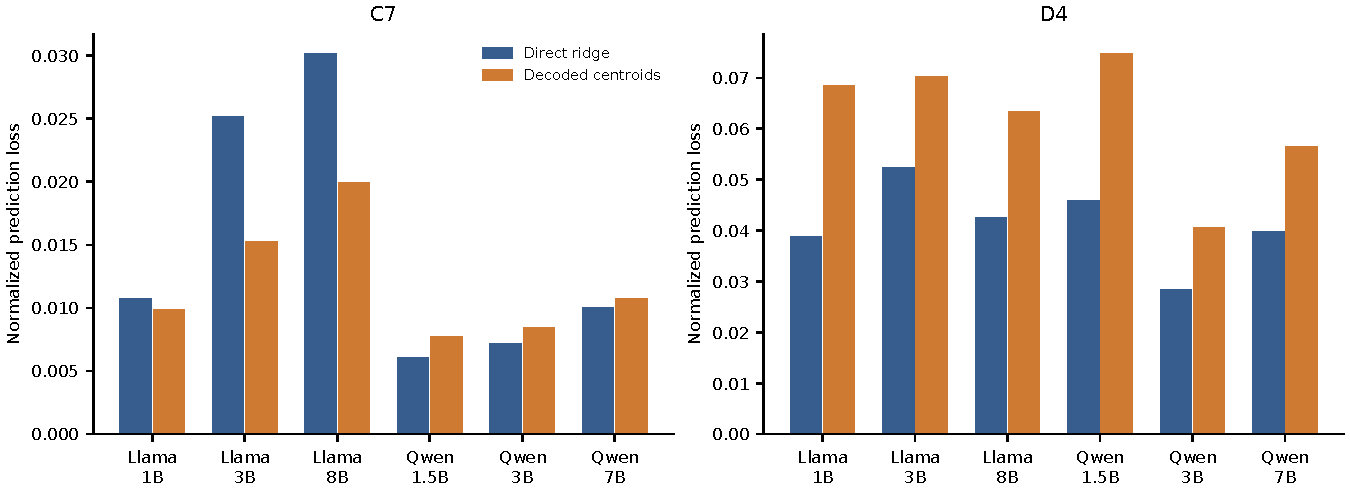
\includegraphics[width=.95\textwidth]{figures/characterization_baselines.pdf}
\caption{All-element prediction: four-readout means for six fixed models. The C7 mean comparison favors decoded centroids in the three Llama models and ridge in the three Qwen models; D4 favors ridge on all six model means. These identities are not independent draws from model lineages. The category comparator has training labels and a known action table. Common PCA and runtime costs are excluded from incremental predictor coordinates.}
\label{fig:characterization-baselines}\end{figure}

\paragraph{What the storage curve measures.}
Primitive-only full fields use 21,504 versus 256 retained coordinates for C7 and 18,432 versus 512 for D4 (84 and 36 times). At the small prescribed budgets they use 256 versus 256 and 480 versus 512. Thus D4 is near-budget, not exactly equal. Farthest-first support selection sees all construction source coordinates but retains only $K$ paired displacements; linear regression compresses all construction target pairs into its coefficients. This original comparison did not fit a compressed nonlinear estimator to all target pairs. The completed RFF/Nystr\"om extension in \cref{app:reproduction} now makes that comparison at explicit parameter budgets; its changed-state/identity handling and selection contract are kept separate from these original values. All 48 full primitive bandwidth selections hit the smallest frozen candidate, $0.125$; some reduced-support selections use $0.25$. These facts bound the comparison and motivate a future development-only grid extension, not retrospective test tuning.

All-element stored ridge maps include an avoidable identity matrix: counts are 1792/2048 for C7/D4, or 1536/1792 after deterministic identity handling. Their $K=14$ fields store 1792/2016, or 1568/1792 after removing zero identity-displacement arrays. C7's original nominal match becomes slightly above-budget after pruning. The common PCA center/basis costs $d(q+1)$ stored float64 coordinates in this export. Training memory, model weights, group tables, centroids, biases, normalization, temporary copies and actual precision must be counted separately for a deployment claim. Retained-coordinate counts are neither total RAM nor statistical capacity.

\paragraph{S3 and context limitations.}
Joint S3 identity prediction loss is $0.018939$, compared with ridge $0.018642$; a small absolute loss is not by itself strong action recovery. The joint context-difference contrast spans zero, and the remaining effects are small relative to the original $0.01$ practical margin. Support displacement reduces prediction loss to $0.015282$ jointly and $0.017580$ on new entities using four extra contexts per entity/state; it is not zero-shot operator superiority. Potential controls were selected in 10/24 conditions (30 split records). Their neural optimization has not been independently replayed. The analytic context fit is separate from that potential. No S3 coordinate-kernel, native intervention or cross-model comparison was added to this original characterization. The subsequent context-predictor and secondary extensions are separately identified in \cref{app:reproduction}.

\paragraph{Audit and provenance boundary.}
The returned archive's checksum, 490-member identity, source/configuration pins, model/readout grid, full metadata banks, exported geometry and 56 frozen intervals were verified. New independent NumPy refits and broader analytic replay reproduced supported coordinate calculations to numerical precision. Historical S3 development selection retains 9,216 reserved cross-block rows per model; exact identities and fitting/scoring masks were checked rather than accepting arbitrary reserved data. The public workflow now validates this historical bank explicitly. Input-feature preprocessing can enumerate nontraining source metadata while assigning zero fitting weight outside training; this is not fitting held-out targets.

The original characterization and its later computational replay are not two independent samples. Compact exports cannot prove original forwards, raw-to-PCA fits, omitted repeated embedding equality or universal prior-access history. Neural Joint/potential refits remain conditional. These limits are recorded with original archive/source hashes and derivative identities in the accompanying release.
